\documentclass[epsfig,10pt,fullpage]{article}

\newcommand{\LabNum}{4}
\newcommand{\CommonDocsPath}{../../common/docs}
\addtolength{\textwidth}{1.5in}
\addtolength{\oddsidemargin}{-0.75in}
\addtolength{\topmargin}{-0.75in}
\addtolength{\textheight}{1.5in}
\addtolength{\evensidemargin}{0.75in}
\setlength\parindent{0pt}
\raggedbottom

\usepackage{ae,aecompl}
\usepackage{epsfig,float,times}
\usepackage[hypcap]{caption}
\usepackage[pdftex, colorlinks]{hyperref}
\usepackage{graphicx}
\usepackage[usenames, dvipsnames]{color}
\usepackage{rotating}
\usepackage{tikz}
\usetikzlibrary{automata,positioning}
\usepackage{placeins}

\widowpenalty 10000
\clubpenalty 10000

\newcommand{\red}[1]{{\color{red}\sf{#1}}}
\newcommand{\green}[1]{{\color{green}\sf{#1}}}
\newcommand{\blue}[1]{{\color{blue}\sf{#1}}}
\definecolor{PineGreen}{rgb}{0.0, 0.47, 0.44}
\definecolor{ForestGreen}{rgb}{0.13, 0.55, 0.13}
\definecolor{Brown}{rgb}{0.59, 0.29, 0.0}

\newcommand{\UPDatePublished}{Oct 2021}
\newcommand{\versnum}{21.1} %version number quartus/AMP
\newcommand{\quartusname}{Quartus\textsuperscript{\textregistered} Prime}	
\newcommand{\UPTextBar}{For \quartusname{} \versnum{}}
\newcommand{\thisyear}{2021 } %for copyright
\newcommand{\company}{FPGAcademy.org}
\newcommand{\longteamname}{FPGAcademy.org}
\newcommand{\teamname}{FPGAcademy}
\newcommand{\website}{FPGAcademy.org}

\newcommand{\productAcronym}{AMP}
\newcommand{\productNameShort}{Monitor Program}

\newcommand{\productNameMedTM}{A Monitor Program}
\newcommand{\productNameMed}{A Monitor Program}

%\newcommand{\headerLogoFilePath}[1]{#1/FPGAcademy.png}

% listings is a package that supports encapsulating source code in LaTeX conveniently
\usepackage{listings}

\def\expandparam\lstinputlisting[#1]#2{\edef\tmp{\noexpand\lstinputlisting[#1]{#2}}\tmp}

%%%%%%%%%%%%%%%%%%%% Source Code Formatting %%%%%%%%%%%%%%%%%%%%
\definecolor{globalCommentColour}{rgb}{0.588,0.588,0.588}

%%%%%%%%%%%%%%%%%%%%%%%%%%%%%%%%%%%%%%%%%%%%%%%%%%%%
% Defining language style
% NiosII ASM
\lstdefinelanguage[NiosII]{Assembler} {
  morekeywords={add, addi, and, andhi, andi, beq, bge, bgeu, bgt, bgtu, ble,  bleu, blt, bltu, bne, br, break,
  bret, call, callr, cmpeq, cmpeqi, cmpge, cmpgei, cmpgeu, cmpgeui, cmpgt, cmpgti, cmpgtu, cmpgtui, cmple,
  cmplei, cmpleu, cmpleui, cmplt, cmplti, cmpltu, cmpltui, cmpne, cmpnei, custom, div, divu, eret, flushd,
  flushda, flushi, flushp, initd, initda, initi, jmp, jmpi, ldb, ldbio, ldbu, ldbuio, ldh, ldhio, ldhu, ldhuio,
  ldw, ldwio, mov, movhi, movi, movia, movui, mul, muli, mulxss, mulxsu, mulxuu, nextpc, nop, nor, or, orhi, ori,
  rdctl, rdprs, ret, rol, roli, ror, sll, slli, sra, srai, srl, srli, stb, stbio, sth, sthio, stw, stwio,
  sub, subi, sync, trap, wrctl, wrtcl, wrprs, xor, xori, xorhi, xori},
  morekeywords=[2]{.abort, .ABORT, .align, .app-file, .ascii, .asciz, .balign, .byte, .comm, .data, .def,
  .desc, .dim, .double, .eject, .else, .end, .endef, .endif, .equ, .equiv, .err, .extern, .file, .fill, .float,
  .global, .globl, .hword, .ident, .if, .include, .int, .irp, .irpc, .lcomm, .lflags, .line, .linkonce, .ln,
  .list, .long, .macro, .mri, .nolist, .octa, .org, .p2align, .psize, .quad, .rept, .sbttl, .scl, .section,
  .set, .short, .single, .size, .sleb128, .skip, .space, .stadb, .stabn, .stabs, .string, .symver, .tag,
  .text, .title, .type, .val, .uleb128, .word},
  morekeywords=[3]{et, bt, gp, sp, fp, ea, sstatus, ra, pc, status, estatus, bstatus, ienable, ipending, cpuid,
  exception, pteaddr, tlbacc, tlbmisc, eccinj, badaddr, config, mpubase, mpuacc},
  sensitive=t,
  alsoletter=.,
  morestring=[b]",
  morecomment=[s]{/*}{*/},
  morecomment=[l]\#,
}[keywords,comments,strings]
   
%% NOTE: morekeywords=[2] are GNU directives.
   
\definecolor{niosInstructionColour}{rgb}{0.000,0.608,0.000}
\definecolor{niosDirectiveColour}{rgb}{0.000,0.000,0.902}
\definecolor{niosSpecialRegColour}{rgb}{0.000,0.000,0.000}
\definecolor{niosStringColour}{rgb}{0.808,0.482,0.000}
   
%% NOTE: To make bold use: =\bfseries\color{<colour>}
\lstdefinestyle{defaultNiosStyle} {
  language=[NiosII]{Assembler},
  stringstyle=\color{niosStringColour},
  keywordstyle=\color{niosInstructionColour},
  keywordstyle=[2]\color{niosDirectiveColour},
  keywordstyle=[3]\itshape\color{niosSpecialRegColour}
}
%%%%%%%%%%%%%%%%%%%%%%%%%%%%%%%%%%%%%%%%%%%%%%%%%%%%

%%%%%%%%%%%%%%%%%%%%%%%%%%%%%%%%%%%%%%%%%%%%%%%%%%%%
% Defining language style
% ArmA9 ASM
\lstdefinelanguage[ArmA9]{Assembler} {
  morekeywords={ADC, ADD, ADDS, AND, ANDS, B, BAL, BEQ, BGE, BGT, BL, BLT, BIC, BKPT, BLX, BNE, BX, CDP, CLZ, CMN, CMP, EOR,
  EORS, LDC, LDM, LDR, LDRB, LDRBT, LDRH, LDRSB, LDRSH, LDRT, LSL, MCR, MLA, MOV, MOVW, MOVT, MRC, MRS, MSR, MUL, MVN, ORR, PLD,
  ROR, RSB, RSC, SBC, SMLAL, SMULL, STC, STM, STR, STRB, STRBT, STRH, STRT, SUB, SUBS, SWI, SWP, SWPB, TEQ, UMLAL,
  PUSH, POP, MOVS, RORS, LSR},
  morekeywords=[2]{.abort, .ABORT, .align, .app-file, .ascii, .asciz, .balign, .byte, .comm, .data, .def,
  .desc, .dim, .double, .eject, .else, .end, .endef, .endif, .equ, .equiv, .err, .extern, .file, .fill, .float,
  .global, .globl, .hword, .ident, .if, .include, .int, .irp, .irpc, .lcomm, .lflags, .line, .linkonce, .ln,
  .list, .long, .macro, .mri, .nolist, .octa, .org, .p2align, .psize, .quad, .rept, .sbttl, .scl, .section,
  .set, .short, .single, .size, .sleb128, .skip, .space, .stadb, .stabn, .stabs, .string, .symver, .tag,
  .text, .title, .type, .val, .vectors, .uleb128, .word},
  morekeywords=[3]{SP, PC, MIDR, CTR, TCMTR, TLBTR, MPIDR, ID_PFR0, ID_PFR1, ID_DFR0, ID_MMFR0, ID_MMFR1, ID_MMFR2,
  ID_MMFR3, ID_ISAR0, ID_ISAR1, ID_ISAR2, ID_ISAR3, ID_ISAR4, CCSIDR, CLIDR, AIDR, CSSELR, TTBR0, TTRB1, TTBR2, DACR,
  DFSR, IFSR, ADFSR, AIFSR, DFAAR, IFAR, ICIALLUIS, BPIALLIS, PAR, ICIALLU, ICIMVAU, BPIALL, DCIMVAC, DCISW, V2PCWPR,
  DCCVAC, DCCSW, DDIMVAC, DCISW, TLBALLIS, TLBIMVAIS, TLBIASIDIS, TLBIMVAAIS, TLBIALL, TLBIMVA, TLBIASID, TLBIMVAA,
  PMCR, PMCNTENSET, PMCNTENCLR, PMOVSR, PMSWINC, PMSELR, PMXEVTYPER, PMXEVCNTR, PMUSERENR, PMINTENSET, PMINTENCLR,
  PRRR, NRRR, PLEIDR, PLEASR, PLEFSR, PLEUAR, PLEPCR, VBAR, MVBAR, ISR, FCSEIDR, CONTEXTIDR, TPIDRURW, TPIDRURO, TPIDRPRW},
  sensitive=f,
  alsoletter=.,
  morestring=[b]",
  morecomment=[s]{/*}{*/},
  morecomment=[l]{//},
}[keywords,comments,strings]
   
%% NOTE: morekeywords=[2] are GNU directives.
   
\definecolor{armInstructionColour}{rgb}{0.000,0.608,0.000}
\definecolor{armDirectiveColour}{rgb}{0.000,0.000,0.902}
\definecolor{armSpecialRegColour}{rgb}{0.000,0.000,0.000}
\definecolor{armStringColour}{rgb}{0.808,0.482,0.000}
   
\lstdefinestyle{defaultArmStyle} {
  language=[ArmA9]{Assembler},
  stringstyle=\color{armStringColour},
  keywordstyle=\color{armInstructionColour},
  keywordstyle=[2]\color{armDirectiveColour},
  keywordstyle=[3]\itshape\color{armSpecialRegColour}
}
%%%%%%%%%%%%%%%%%%%%%%%%%%%%%%%%%%%%%%%%%%%%%%%%%%%%

%%%%%%%%%%%%%%%%%%%%%%%%%%%%%%%%%%%%%%%%%%%%%%%%%%%%
% Defining language style
% FPGAcademy ASM
\lstdefinelanguage{ASM}{
  morekeywords = [1]{mv, mvt, mvne, mvcc, add, sub, st, ld, and, b, bne, beq, bcc, bcs},
  morekeywords = [2]{word, define},
  keywordstyle = [1]\color{ForestGreen},
  keywordstyle = [2]\color{blue},
  sensitive = true,
  morecomment = [l]{//},
}

\lstset{
  language = ASM,
  basicstyle=\small\color{black}\ttfamily,
  commentstyle=\small\color{Brown}\itshape\ttfamily,
  showstringspaces=false,
  frame=none, %lines % boxed listings
  breaklines=true,
  breakatwhitespace=true,
  tabsize=3
}
%%%%%%%%%%%%%%%%%%%%%%%%%%%%%%%%%%%%%%%%%%%%%%%%%%%%

%%%%%%%%%%%%%%%%%%%%%%%%%%%%%%%%%%%%%%%%%%%%%%%%%%%%
% Defining language style
% Java
\definecolor{javaStringColour}{rgb}{0.808,0.482,0}
%%%%%%%%%%%%%%%%%%%%%%%%%%%%%%%%%%%%%%%%%%%%%%%%%%%%

%%%%%%%%%%%%%%%%%%%%%%%%%%%%%%%%%%%%%%%%%%%%%%%%%%%%
% Defining language style
% C
\definecolor{CStringColour}{rgb}{0.808,0.482,0}

\lstset{
  language = C,
  basicstyle=\small\color{black}\ttfamily, 
  commentstyle=\small\color{PineGreen}\itshape\ttfamily,
  keywordstyle=\small\color{blue}\bfseries\ttfamily,
  showstringspaces=false,
  frame=none, %lines % boxed listings
  breaklines=true,
  breakatwhitespace=true,
  tabsize=3
}
%%%%%%%%%%%%%%%%%%%%%%%%%%%%%%%%%%%%%%%%%%%%%%%%%%%%

%%%%%%%%%%%%%%%%%%%%%%%%%%%%%%%%%%%%%%%%%%%%%%%%%%%%
% Defining language style
% Verilog
\definecolor{verilogCommentColour}{rgb}{0.000,0.502,0.000}

\lstdefinestyle{defaultVerilogStyle} {
  language={Verilog},
  keywordstyle=\color{blue},
  commentstyle=\color{verilogCommentColour}
}
%%%%%%%%%%%%%%%%%%%%%%%%%%%%%%%%%%%%%%%%%%%%%%%%%%%%

%%%%%%%%%%%%%%%%%%%%%%%%%%%%%%%%%%%%%%%%%%%%%%%%%%%%
% Defining language style
% VHDL
\lstdefinestyle{defaultVHDLStyle} {
  language={VHDL},
  keywordstyle=\color{blue},
  commentstyle=\color{verilogCommentColour}
}
%%%%%%%%%%%%%%%%%%%%%%%%%%%%%%%%%%%%%%%%%%%%%%%%%%%%

%%%%%%%%%%%%%%%%%%%%%%%%%%%%%%%%%%%%%%%%%%%%%%%%%%%%
% Defining language style
% LaTeX
\lstdefinelanguage[LocalLaTeX]{TeX}[LaTeX]{TeX}{moretexcs={bf, it, sf, lstset},}

\lstdefinestyle{defaultLocalLatexStyle} {
  language=[LocalLatex]{TeX},
  keywordstyle=\color{blue}\bfseries,
  keywordstyle=[2]\color{blue},
  keywordstyle=[3]\color{blue}\bfseries
}
%%%%%%%%%%%%%%%%%%%%%%%%%%%%%%%%%%%%%%%%%%%%%%%%%%%%

%%%%%%%%%%%%%%%%%%%%%%%%%%%%%%%%%%%%%%%%%%%%%%%%%%%%
% Defining language style
% Default
\lstset{
  basicstyle=\small\color{black}\ttfamily,
  commentstyle=\small\color{globalCommentColour}\itshape\ttfamily,
  keywordstyle=\small\color{blue}\bfseries\ttfamily,
  showstringspaces=false,
  frame=none, %lines % boxed listings
  breaklines=true,
  breakatwhitespace=true,
  tabsize=3
}
%%%%%%%%%%%%%%%%%%%%%%%%%%%%%%%%%%%%%%%%%%%%%%%%%%%%


\hypersetup{
  pdftitle={OpenCL Lab Exercise \LabNum},
  linkcolor=blue,
  hyperindex=true,
  pdfauthor={FPGAcademy.org},
  pdfkeywords={FPGAcademy.org, FPGAcademy, Lab, Exercise, OpenCL},
  bookmarks,
  bookmarksopen=false,
  filecolor=blue,
  pdfstartview={FitH},
  urlcolor=blue,
  plainpages=false,
  pdfpagelabels=true,
  linkbordercolor={1 1 1} %no color for link border
}



\begin{document}

\centerline{\huge OpenCL}
~\\
\centerline{\huge Laboratory Exercise \LabNum}
~\\
\centerline{\large Classification of Handwritten Digits using Machine Learning: Linear Classifier}
~\\

In this exercise you will learn about a machine learning approach to classifying handwritten digits.
You will create software and hardware implementations of a linear classifier that accepts images of handwritten digits ranging 0 to 9 and determines which digit is present in each image.

\section*{The MNIST Handwritten Digits Database}

In this exercise you will use the MNIST handwritten digits database,  
which is widely used by scientists around the world to train and test handwritten digit recognition machines. 
The database provides 28x28-pixel 8-bit grayscale images, each containing a single handwritten digit ranging 0 to 9. An example of
an image from the MNIST database is shown in Figure~\ref{fig:mnist_image}.

\begin{figure}[H]
   \begin{center}
       \hspace*{1.5cm}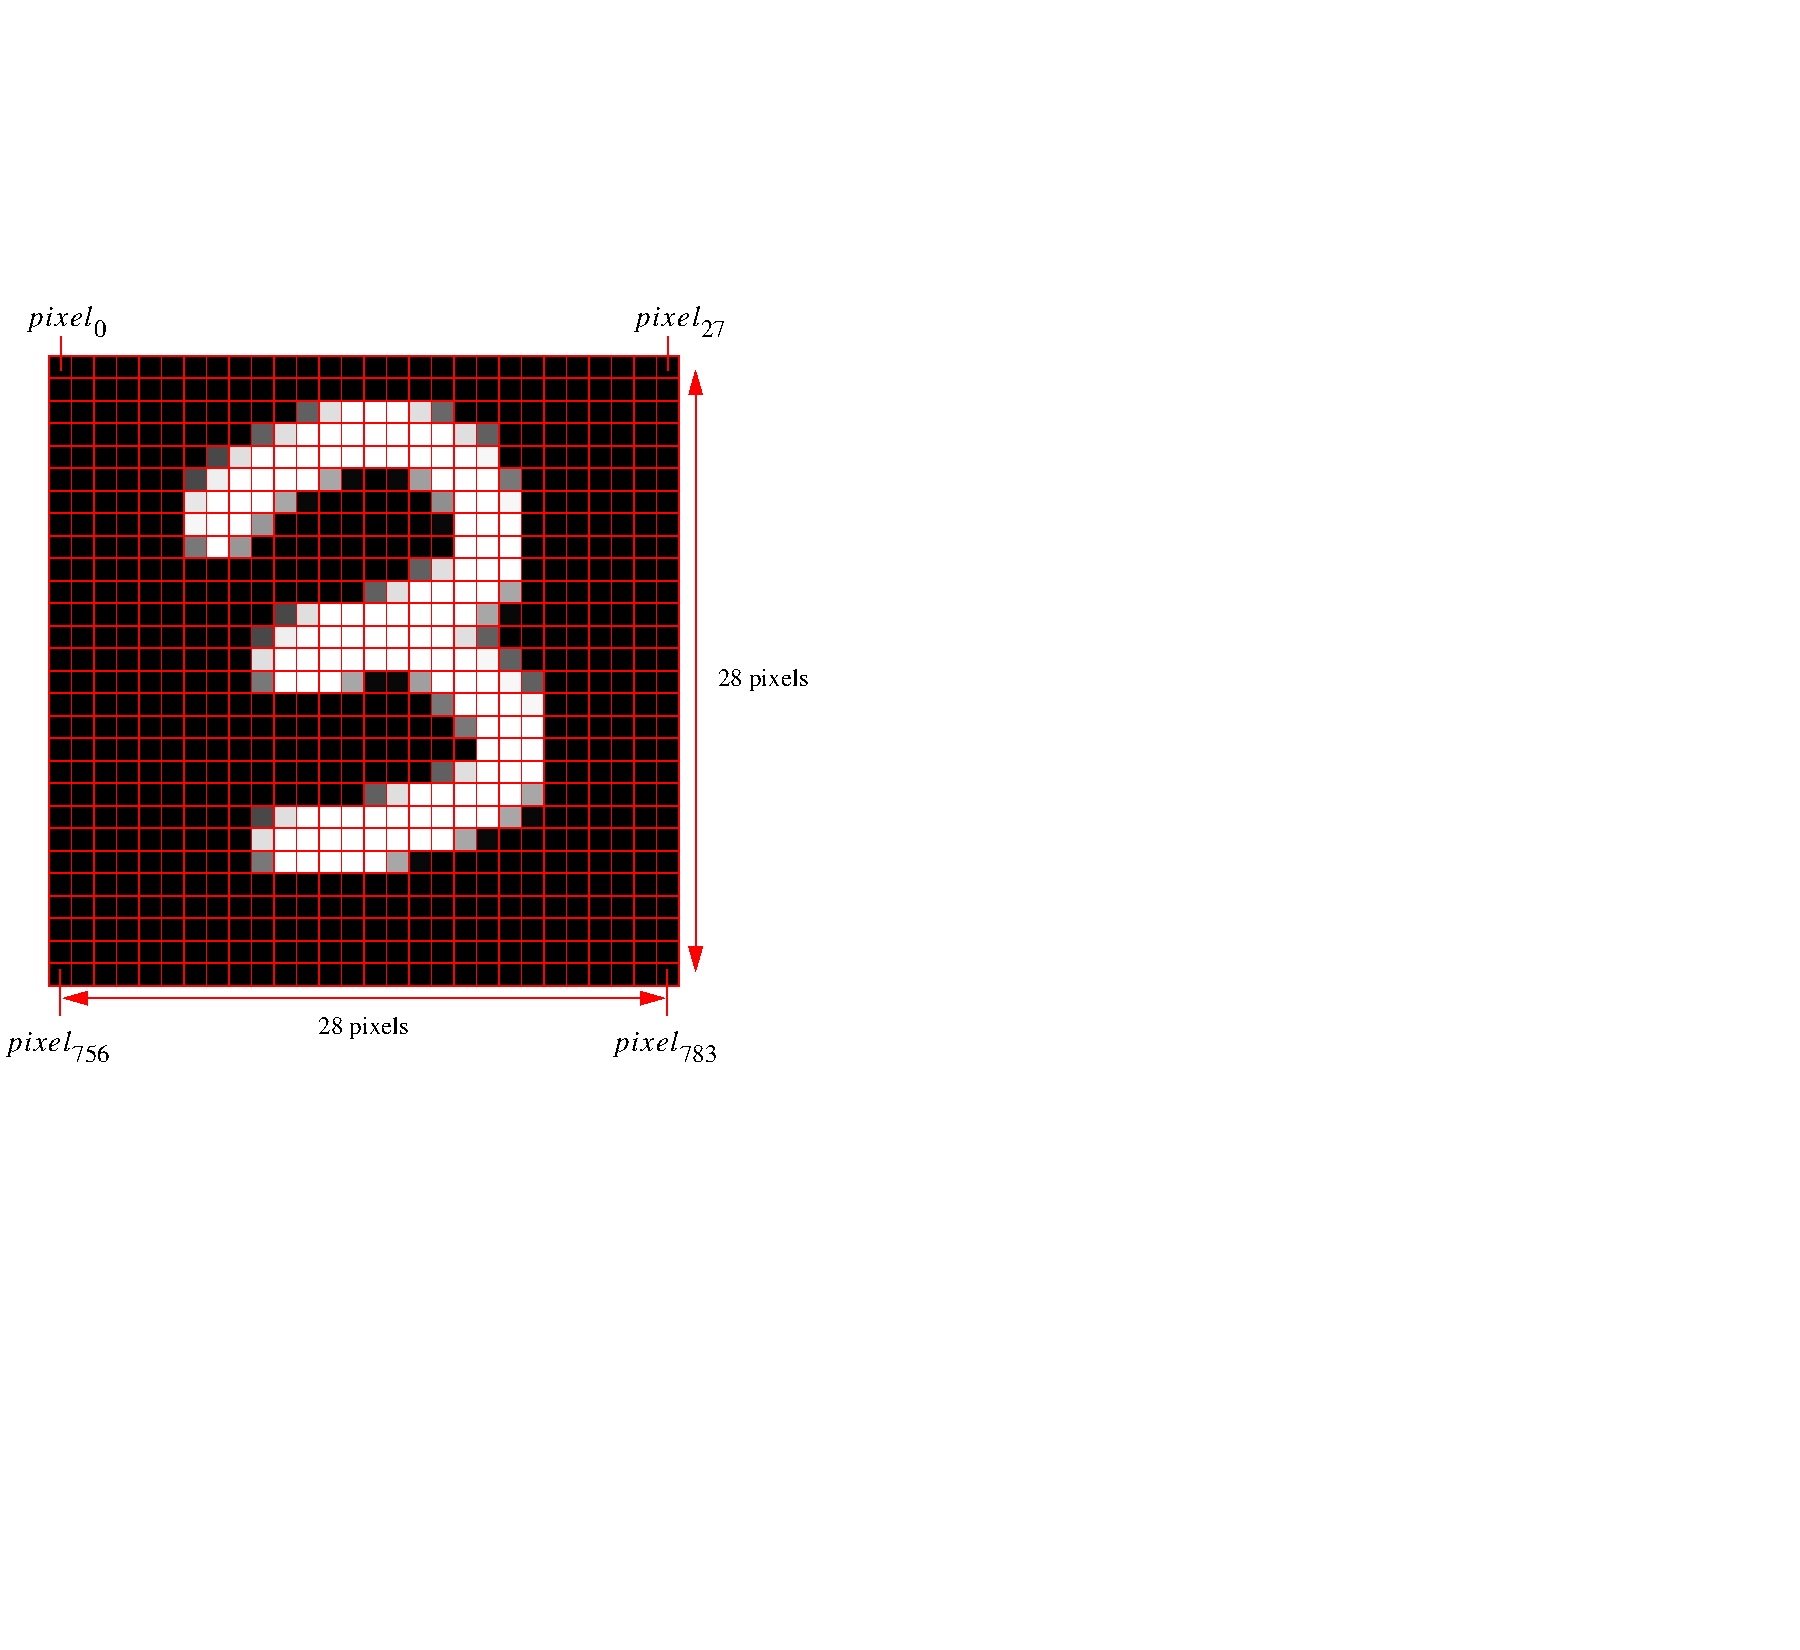
\includegraphics[scale=0.7]{figures/fig_mnist_image}
   \end{center}
   \caption{An example handwritten digit image from the MNIST database}
	\label{fig:mnist_image}
\end{figure}

The database contains a training set of 60000 images which are used to train the classifier, and a test set of 10000 images which are used to test the classifier's accuracy. 
The 60000 training images have already been used to train the weights for the linear classifier. 
Your task is to use the provided weights to implement the linear classifier and test its classification accuracy on the 10000 test images.

\section*{The Linear Classifier}

\begin{figure}[H]
   \begin{center}
       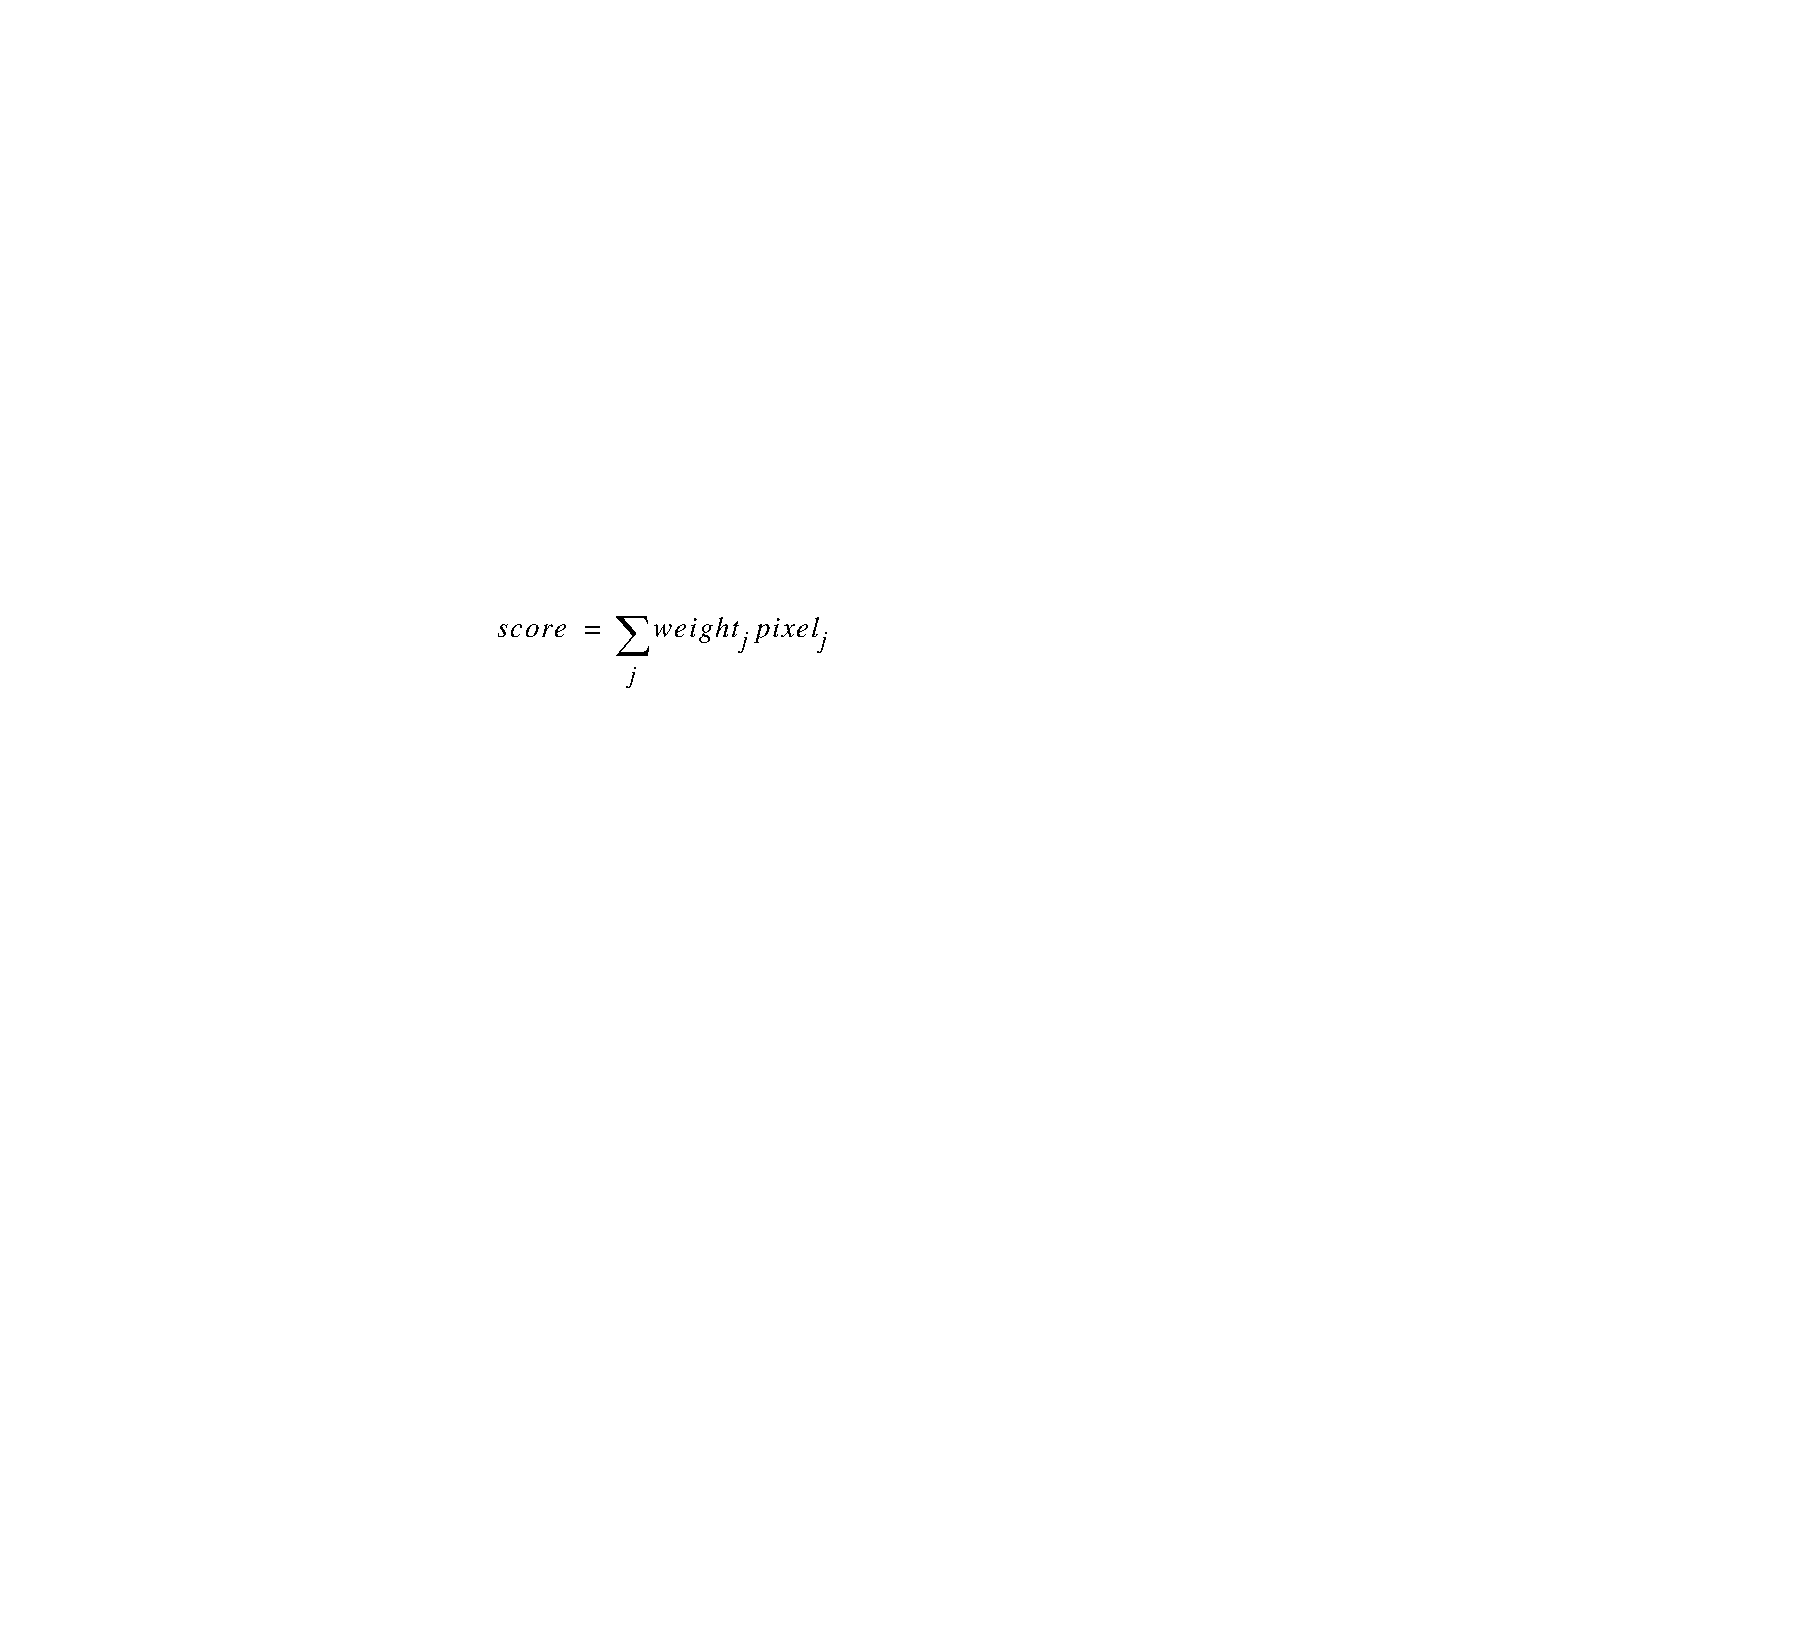
\includegraphics[scale=1]{figures/fig_linear_classifier_equation}
   \end{center}
   \caption{The equation for calculating the score of a class in the linear classifier}
	\label{fig:linear_classifier_equation}
\end{figure}

The linear classifier evaluates the likelihood (or score) of the input image being each of the possible digits.
The score is calculated using the equation shown in Figure~\ref{fig:linear_classifier_equation}, where j ranges 0 to 783 to span the pixels and their corresponding weights.
Each digit has its own set of weights leading to a total of 10*784 = 7840 weights for the classifier.
After calculating the scores of all the digits, the digit whose score is highest is chosen as the classification result. 
An example of the calculations is shown in Figure~\ref{fig:linear_classifier}, where the linear classifier receives an input image containing the digit 3 and
outputs the correct classification result.


\begin{figure}[H]
   \begin{center}
       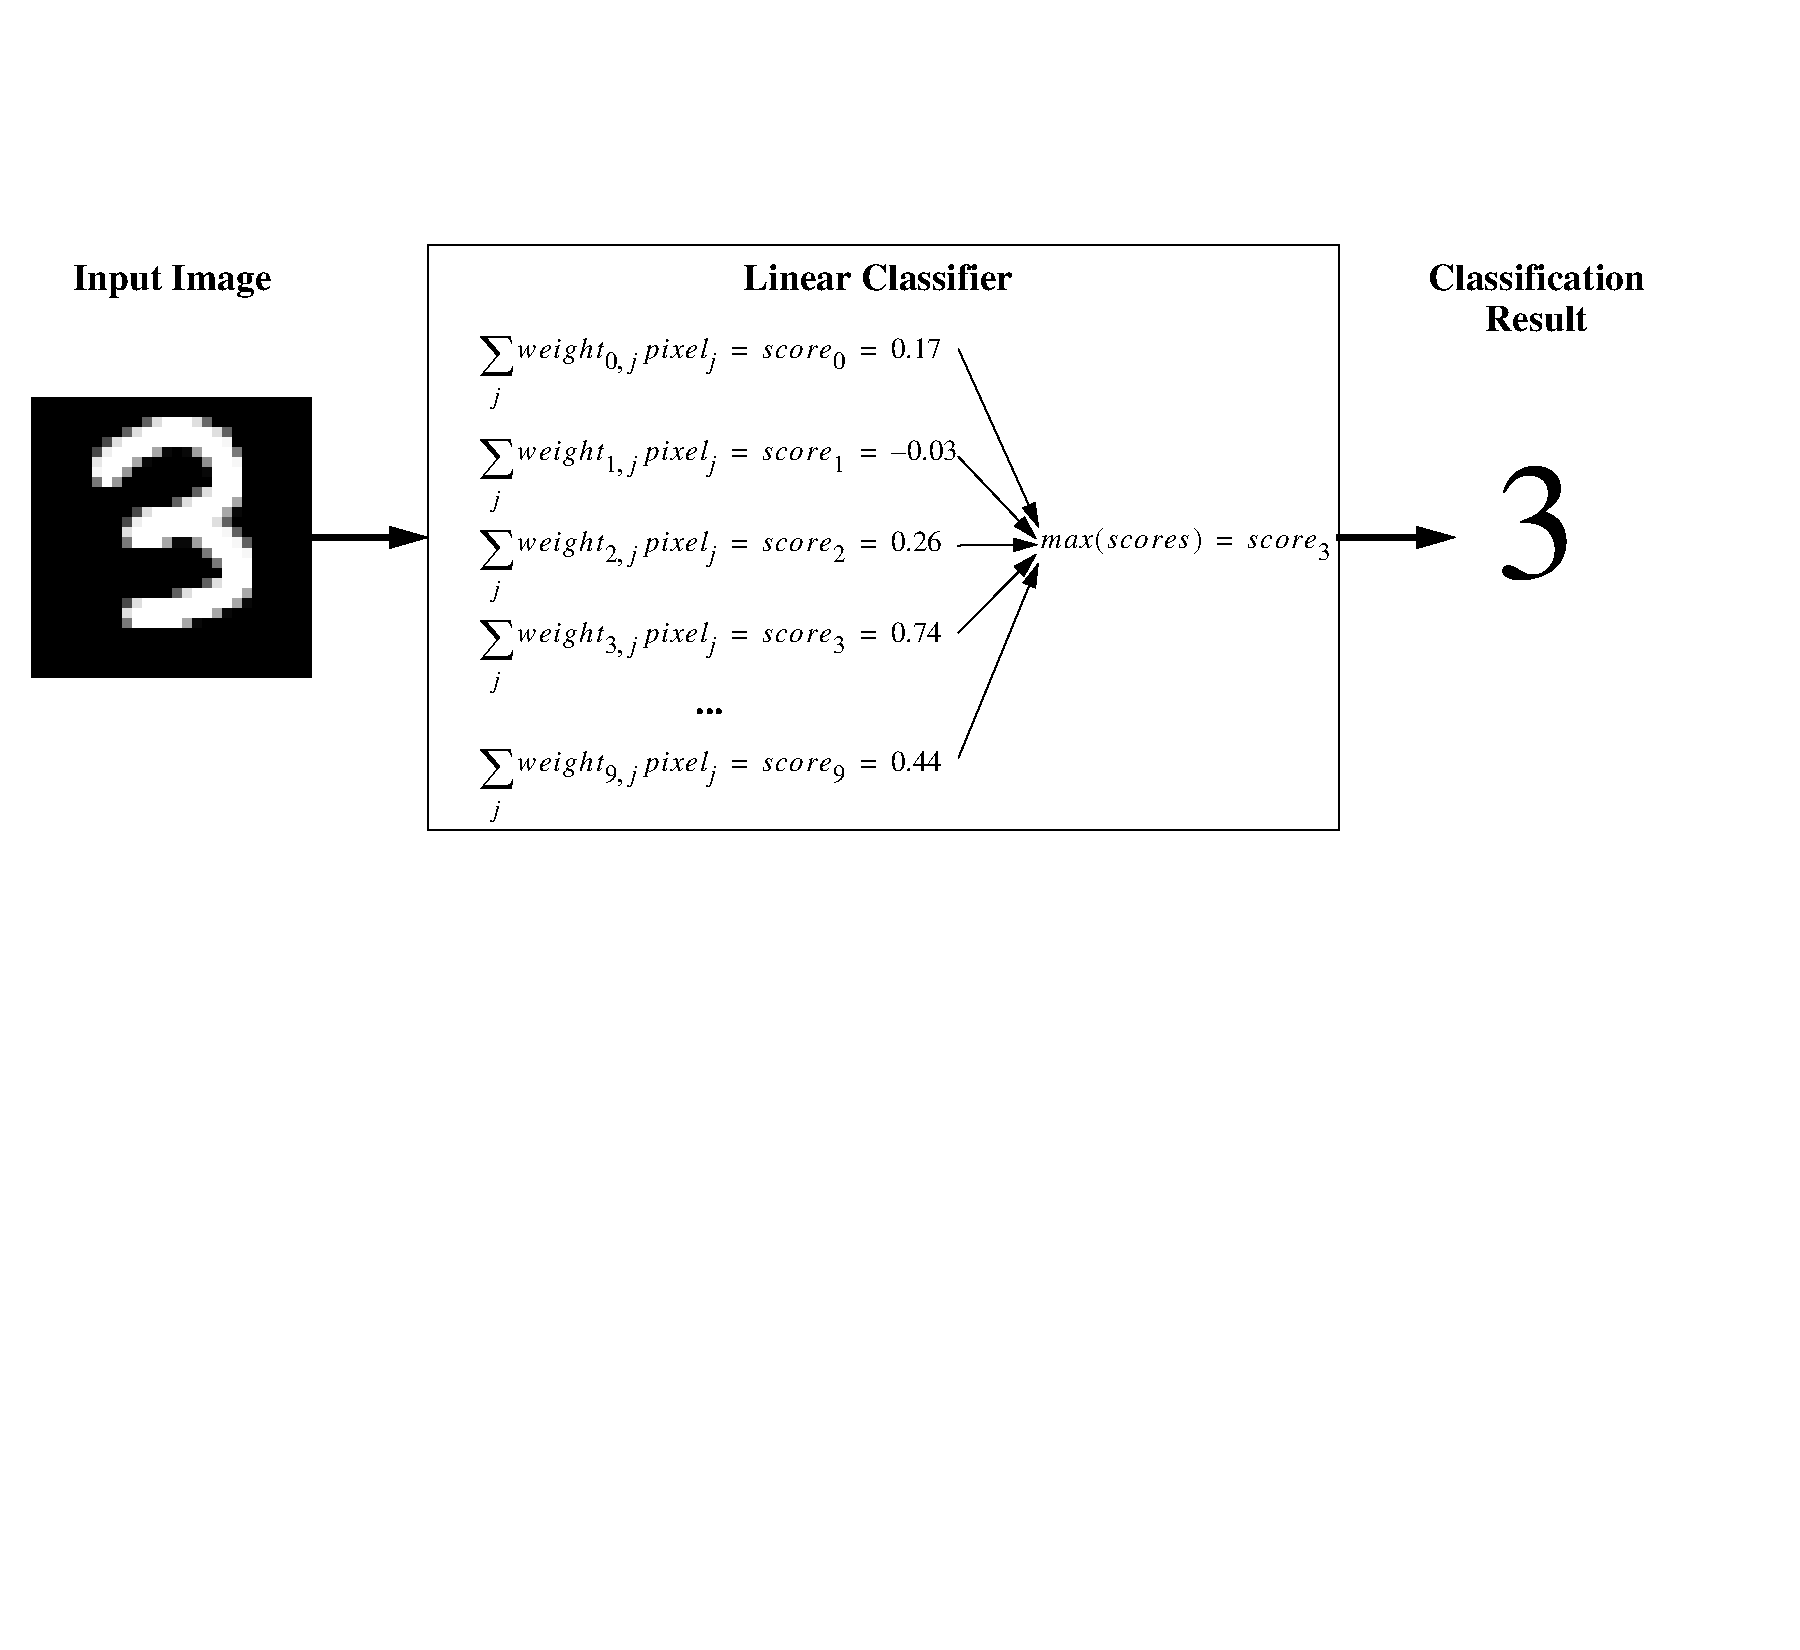
\includegraphics[scale=0.58]{figures/fig_linear_classifier}
   \end{center}
   \caption{The linear classifier operating on an input image containing the digit ``3'' and yielding the correct result}
	\label{fig:linear_classifier}
\end{figure}


\section*{Part I}
\noindent
Implement a program in the C++ language that performs linear classification of MNIST handwritten digits. 
Your program must use the trained weights stored in files \textit{weights\_0}, \textit{weights\_1}, ... , \textit{weights\_9}, in the \textit{/design\_files/weights\_fp/} directory. 
Test your program by classifying the 10000 MNIST test images stored in the file \textit{/design\_files/t10k-images-idx3-ubyte}. 
Compare the results of your classifier to the correct labels stored in the file \textit{/design\_files/t10k-labels-idx1-ubyte} to calculate
your classifier's accuracy as: \[Accuracy = (\#\ of\ correct\ results )/ 10000 * 100\% \]
Compile and execute your program on a DE-Series Linux platform.
Upon completion, your program should output the classification accuracy and the runtime in milliseconds.

\subsubsection*{Parsing the MNIST Database Files}
The MNIST database is provided in .idx files. The file formats of the MNIST images and labels files are shown in Figure~\ref{fig:mnist_file_format}. 
Your program must open and parse these files to extract the image pixels and labels. Each pixel is 8 bits and represents a grayscale value.
Each label is also 8 bits, and its value can range from 0 to 9 to indicate the correct classification of the corresponding image.
The 32-bit integers stored in these files are stored in most-significant byte (MSB)-first format, which
must first be converted to least significant byte (LSB)-first format before being used on the ARM processors of the DE-series boards.

\lstset{}
\begin{figure}[H]
\begin{center}
\begin{minipage}[t]{12.7 cm}
\begin{lstlisting}
TEST SET IMAGE FILE (t10k-images-idx3-ubyte):
[offset] [type]          [value]          [description] 
0000     32 bit integer  0x00000803(2051) magic number 
0004     32 bit integer  10000            number of images 
0008     32 bit integer  28               number of rows 
0012     32 bit integer  28               number of columns 
0016     unsigned byte   ??               pixel 
0017     unsigned byte   ??               pixel 
........ 
xxxx     unsigned byte   ??               pixel

TEST SET LABEL FILE (t10k-labels-idx1-ubyte):
[offset] [type]          [value]          [description] 
0000     32 bit integer  0x00000801(2049) magic number (MSB first) 
0004     32 bit integer  10000            number of items 
0008     unsigned byte   ??               label 
0009     unsigned byte   ??               label 
........ 
xxxx     unsigned byte   ??               label
The labels values are 0 to 9.
\end{lstlisting}
\end{minipage}
\end{center}
\vspace{-.23in}\caption{File formats of the MNIST files. Source: http://yann.lecun.com/exdb/mnist/}
\label{fig:mnist_file_format}
\end{figure}

\subsubsection*{Parsing the Weights Files}

Trained weights for use in this part of the exercise are provided in the directory \textit{/design\_files/weights\_fp/}. There are 10 weights files named 
\textit{weights\_0}, \textit{weights\_1}, ... , \textit{weights\_9} that correspond to their respective digits.
Each file contains 784 32-bit floating point weights that can be parsed using the code shown in 
Figure~\ref{fig:parse_weights_code}. 

\lstset{language=C++}
\begin{figure}[H]
\begin{center}
\begin{minipage}[t]{16 cm}
\begin{lstlisting}
#define FEATURE_COUNT 784

// weights must be an array of sufficient size (>= 784)
bool read_weights_file(char *filename, float *weights) {
	FILE *f = fopen(filename, "rb");
	if (f == NULL){
		printf("ERROR: could not open %s\n",filename);
		return false;
	}
	int read_elements = fread(weights, sizeof(float), FEATURE_COUNT, f);
	fclose(f);
	
	if (read_elements != FEATURE_COUNT){
		printf("ERROR: read incorrect number of weights from %s\n", filename);
		return false;
	}
	return true;
}
\end{lstlisting}
\end{minipage}
\end{center}
\vspace{-0.33in}\caption{Function that parses a weights file}
\label{fig:parse_weights_code}
\end{figure}

\section*{Part II}

Implement an OpenCL kernel that performs linear classification of handwritten digits. Use the function prototype shown in Figure~\ref{fig:kernel_v1}. 
The kernel reads the input array \texttt{images} which contains 10000 images. Each image in the array is 784 chars long, for a total of 10000 * 784 = 7840000 chars in the array.
The kernel reads the input array \texttt{weights} which contains 10 sets of 784 weights, for a total of 7840 floats in the array. 
The kernel writes the classification results to the output array \texttt{results} which will contain 10000 chars when the kernel finishes.
Each char in the \texttt{results} array will contain a value from 0 to 9 indicating the classification result.

\lstset{}
\begin{figure}[H]
\begin{center}
\begin{minipage}[t]{16 cm}
\vspace{-0.13in}\begin{lstlisting}
__attribute__((reqd_work_group_size(10000,1,1)))
__kernel void linear_classifier(global const unsigned char * restrict images, 
								constant float * restrict weights,
								global unsigned char * restrict results)
{
	... Your Code ...
}
\end{lstlisting}
\end{minipage}
\end{center}
\vspace{-0.33in}\caption{Function prototype for the linear classifier kernel}
\label{fig:kernel_v1}
\end{figure}

In previous exercises you manually created local memories to cache frequently used values and reduce memory access overhead.
In this exercise, you will use Intel FPGA SDK for OpenCL's automatic cache generation feature to cache the linear classifier's weights. 
This is done by assigning the \texttt{constant} 
keyword to the weights array which tells the compiler that the values in the array are constant and should be cached to improve performance.
By default the Intel FPGA SDK for OpenCL creates a cache that is 16384 bytes large to store the values. 
The cache size can be changed when compiling your kernel
using the argument \texttt{-const-cache-bytes=<N>}, where <N> is the number of bytes desired. 
Select a cache size that is sufficiently large to minimize cache misses.

~\\
Maximize the performance of your design by unrolling your loop(s) until you run out of FPGA resources.
Modify the SW implementation from Part I to invoke your OpenCL kernel. 
Ensure that your OpenCL kernel produces the same classification accuracy as your software implementation in Part I. 
Determine the runtime of your OpenCL kernel. How does its performance compare to that of the software implementation?

\section*{Part III}

Open the ``Area Analysis of System'' page in the compilation report of your design in Part II. By examining the detailed breakdowns, 
you will see that the majority of resource utilization comes from implementing floating-point arithmetic operations. 
How many ALUTs, FFs, and DSPs does a floating-point add require? How many ALUTs, FFs, and DSPs does a floating-point multiply require?
How many floating-point add operations could you fit into your FPGA, assuming you are implementing nothing else? 
How many floating-point multiply operations could you fit into your FPGA, assuming you are implementing nothing else?
Note that you can get the total number of available ALUTs, FFs, and DSPs on the ``Summary'' page of the report. 

\section*{Part IV}

In this part of the exercise, you will modify your implementation from Part II to use fixed-point arithmetic instead of
floating-point arithmetic. 


\subsubsection*{Fixed-Point Arithmetic}

The fixed-point datatype stores real numbers using a fixed number of digits after the decimal point. 
Fixed-point data consists of an arbitrary number of bits which are divided into two sets. 
The set of most significant bits represents the whole number to the left of the decimal point,
while the set of least significant bits represents the fractional portion to the right of the decimal point.
As an example, a 16-bit fixed-point number can be divided into a 12-bit set and an 4-bit set, where the most
significant 12 bits represent the whole number, and the least significant 4 bits represent the fractional number. 
Such a fixed-point representation is called ``12.4 fixed-point format''.
Each bit contributes 2\textsuperscript{x} to the real number value, where x is the bit's position offset from the decimal point. 
Figure~\ref{fig:fixed_point} shows an example of a 16-bit value which is interpreted as a 12.4 fixed-point value and as a 8.8 fixed-point value.

\begin{figure}[H]
   \begin{center}
       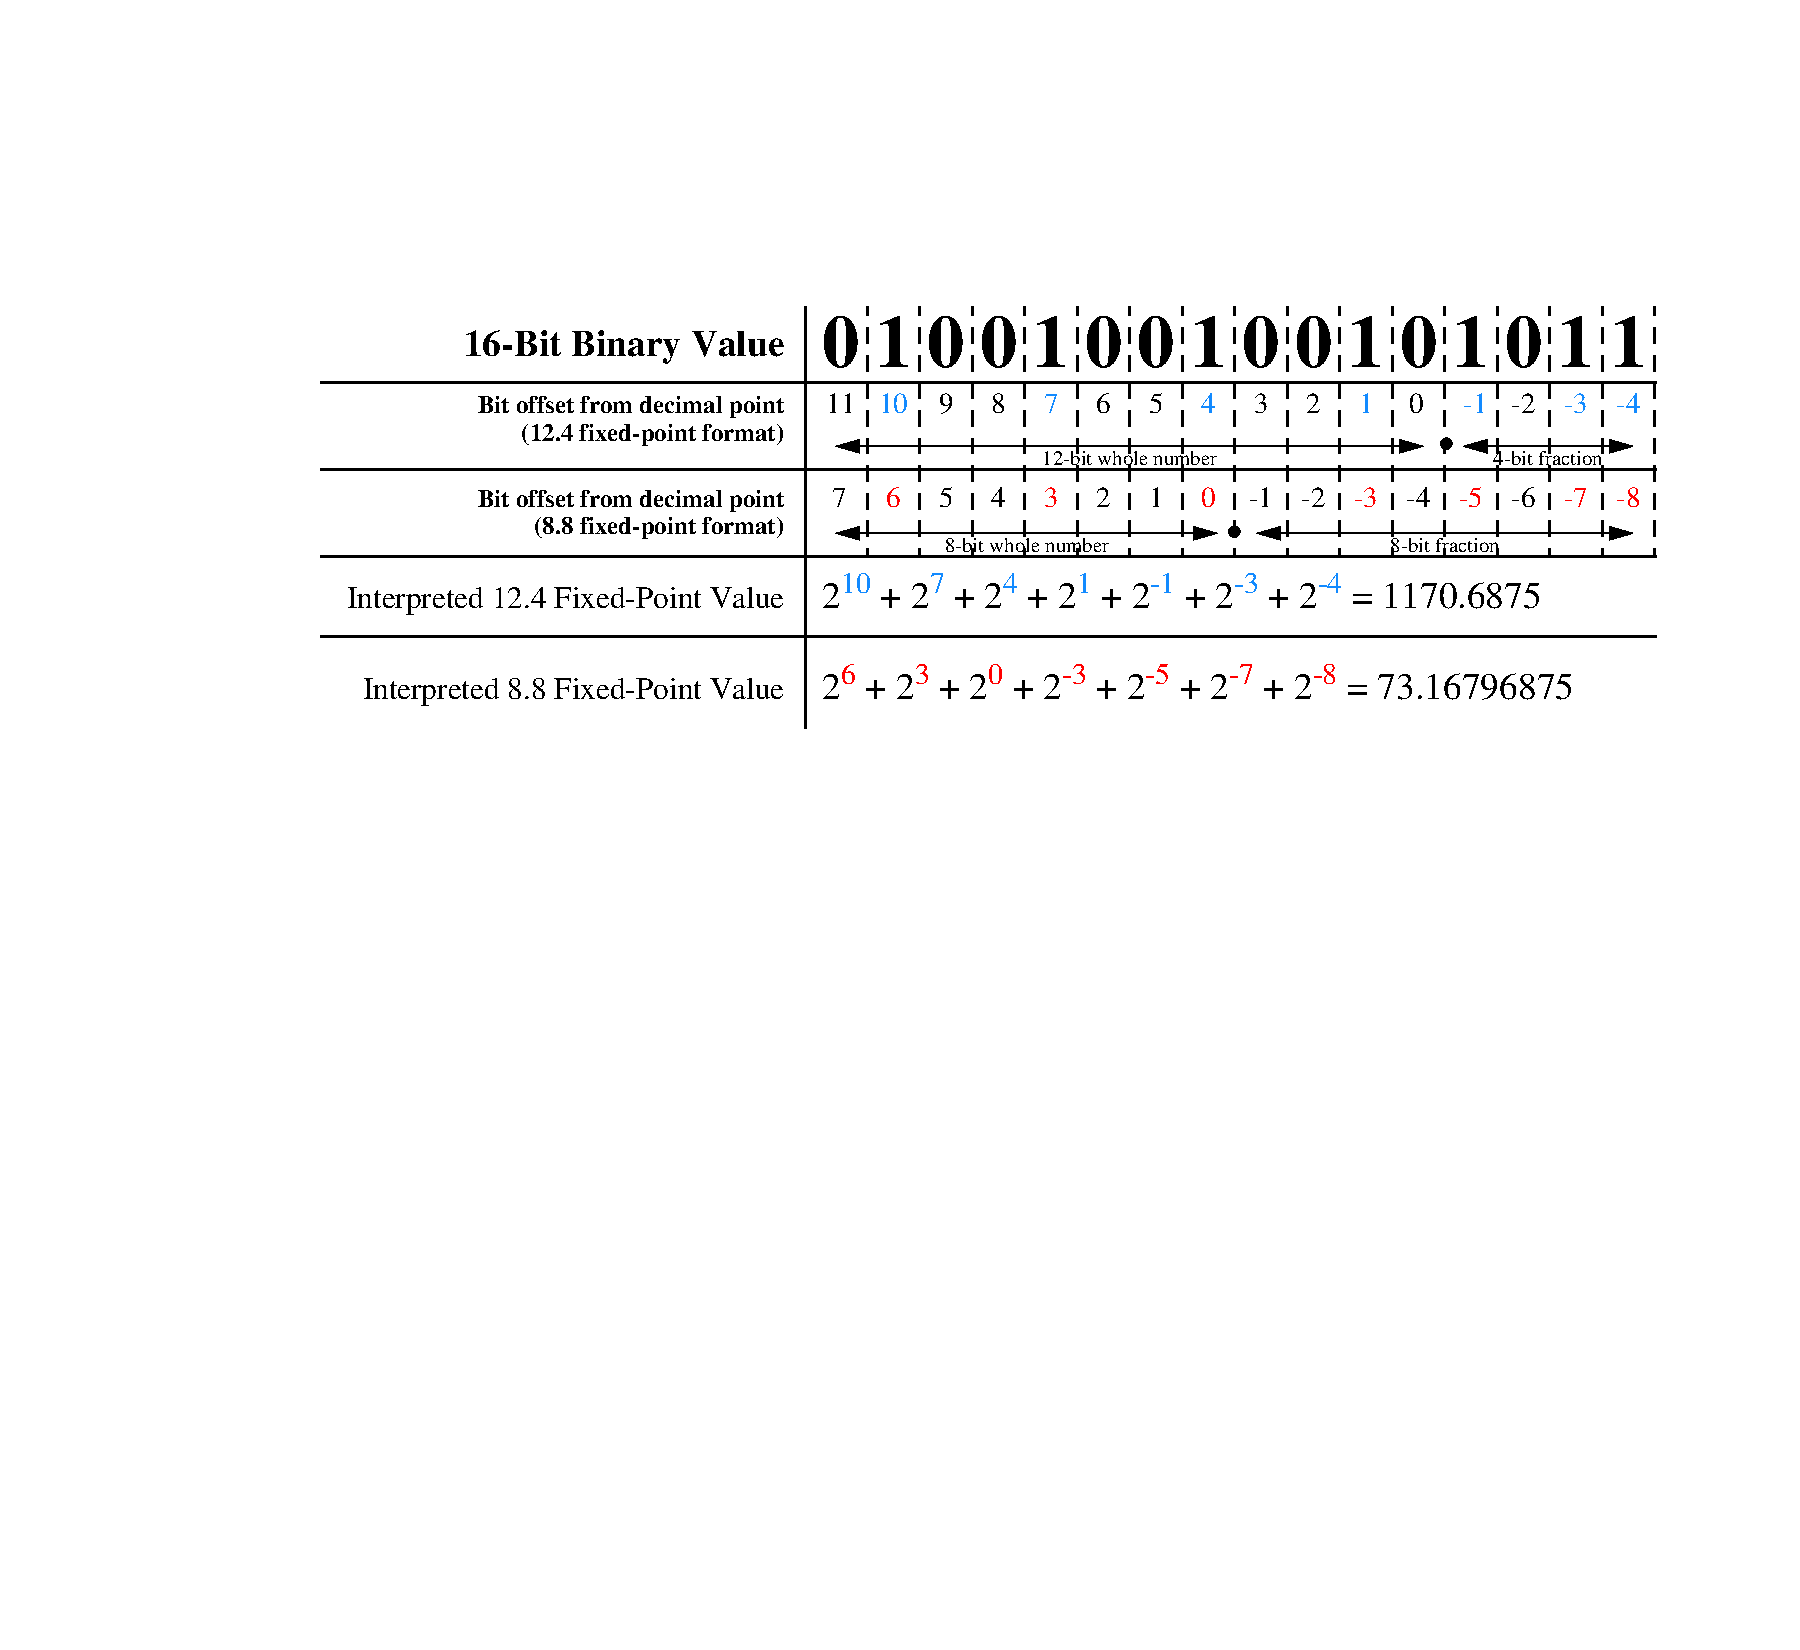
\includegraphics[scale=0.70]{figures/fig_fixed_point}
   \end{center}
   \caption{Interpreting a 16-bit value as 12.4 and 8.8 fixed-point values}
	\label{fig:fixed_point}
\end{figure}

An advantage of using fixed-point arithmetic is that the operations require fewer hardware resources to implement 
compared to floating-point arithmetic. 

~\\
This means that a fixed-point circuit can be smaller and more power-efficient than its floating-point equivalent. 
Alternatively, you could achieve higher performance by implementing more fixed-point units with the same hardware resources.

~\\
Fixed-point multiplication can be computed using an integer multiplier circuit, with the caveat that the circuit
does not track the decimal point locations of the multiplicands and the product. 
It is therefore the designer's responsibility to track the decimal point locations.
The product's decimal point location (offset from the LSB) is determined by adding the offsets in the multiplicands.
For example, if you multiply a 12.4 fixed-point number by a 8.8 fixed-point number, the decimal point in the product
will be offset from the LSB by 4 + 8 = 12 bits. In other words, the product would have a 12-bit fraction.

~\\
Fixed-point addition can be computed using an integer adder circuit, provided that two summands have the same decimal point location. 
When adding two fixed-point values whose decimal point locations differ, one of the summands must be shifted to match the other prior to addition.
The resulting sum will have the same decimal point location as its summands.


\subsubsection*{Modifying Your Kernel to Use Fixed-Point Arithmetic}

Modify your host program to parse the fixed-point weights in the directory \textit{/design\_files/weights\_fxp/}.
These fixed-point weights are stored in 16.16 fixed-point format. 
Modify your kernel to accept the fixed-point weights as an \texttt{int} array, as shown in Figure~\ref{fig:kernel_v2}. 
When multiplying the 16.16 fixed-point weights by the 8-bit pixels, the pixels can be considered to be
8.0 fixed-point numbers. 


\lstset{language=C}
\begin{figure}[H]
\begin{center}
\begin{minipage}[t]{16 cm}
\begin{lstlisting}
__attribute__((reqd_work_group_size(10000,1,1)))
__kernel void linear_classifier(global const unsigned char * restrict images, 
								constant int * restrict weights,
								global unsigned char * restrict results)
{
	... Your Code ...
}
\end{lstlisting}
\end{minipage}
\end{center}
\vspace{-0.33in}\caption{Function prototype for the linear classifier kernel that uses fixed point weights}
\label{fig:kernel_v2}
\end{figure}

Use the \texttt{aoc} flag \texttt{-c} to obtain a compilation report for your modified kernel and examine the resource utilization of
implementing fixed-point addition and multiplication. Determine the per-adder and per-multiplier resource cost and compare them 
to the numbers you determined in Part III.
Unroll your loops to fully utilize the resources of the FPGA and maximize the kernel's performance.
How many times can you unroll your loop before running out of resources, and how does that compare to your design from Part II?
Compile your design and use it to classify the MNIST test images.
What is the runtime of your new kernel and how does it compare to that of your kernel from Part II?
Is your classification accuracy affected? Why or why not? In what situations would changing from
floating-point arithmetic to fixed-point arithmetic affect (and not affect) classification accuracy?


%%%%%%%%%%%%%%%%%%%%%%%%%%%%%%%%%%%%%%%%
%%% FPGAcademy Copyright Information %%%
%%%%%%%%%%%%%%%%%%%%%%%%%%%%%%%%%%%%%%%%

%Always put the copyright on a new page (clear page), with some vertical space from top
\clearpage
\vspace{1in}

\noindent

Copyright {\copyright} FPGAcademy.org. All rights reserved. FPGAcademy and the 
FPGAcademy logo are trademarks of FPGAcademy.org.  This document is provided 
"as is", without warranty of any kind, express or implied, including but not 
limited to the warranties of merchantability, fitness for a particular purpose 
and noninfringement. In no event shall the authors or copyright holders be 
liable for any claim, damages or other liability, whether in an action of 
contract, tort or otherwise, arising from, out of or in connection with the 
document or the use or other dealings in the document.
~\\
~\\
**Other names and brands may be claimed as the property of others.


\end{document}
